\documentclass[12pt, a4paper]{article}
\usepackage{caption}
\usepackage{graphicx}
\usepackage{hyperref}
\hypersetup{
    colorlinks,
    citecolor=black,
    filecolor=black,
    linkcolor=black,
    urlcolor=black
}
\usepackage{tikz-network}
\usepackage{amsmath, amsfonts, amssymb, amsthm}
\usepackage{algpseudocode}
\usepackage{algorithm}
\title{Network and Cybersecurity\\ Assignment 1}
\date{2022}
\author{Kristoffer Klokker}

\usepackage{xcolor,listings}
\usepackage{textcomp}
\usepackage{color}
\usepackage{listings}
\definecolor{codegreen}{rgb}{0,0.6,0}
\definecolor{codegray}{rgb}{0.5,0.5,0.5}
\definecolor{codepurple}{HTML}{C42043}
\definecolor{backcolour}{HTML}{F2F2F2}
\definecolor{bookColor}{cmyk}{0,0,0,0.90}  
\color{bookColor}
\setcounter{tocdepth}{1}
\lstset{upquote=true}

\lstdefinestyle{mystyle}{
    backgroundcolor=\color{backcolour},   
    commentstyle=\color{codegreen},
    keywordstyle=\color{codepurple},
    numberstyle=\numberstyle,
    stringstyle=\color{codepurple},
    basicstyle=\footnotesize\ttfamily,
    breakatwhitespace=false,
    breaklines=true,
    captionpos=b,
    keepspaces=true,
    numbers=left,
    numbersep=10pt,
    showspaces=false,
    showstringspaces=false,
    showtabs=false,
    tabsize=3,
}
\lstset{style=mystyle}
\usepackage{zref-base}

\makeatletter
\newcounter{mylstlisting}
\newcounter{mylstlines}
\lst@AddToHook{PreSet}{%
  \stepcounter{mylstlisting}%
  \ifnum\mylstlines=1\relax
    \lstset{numbers=none}
  \else
    \lstset{numbers=left}
  \fi
  \setcounter{mylstlines}{0}%
}
\lst@AddToHook{EveryPar}{%
  \stepcounter{mylstlines}%
}
\lst@AddToHook{ExitVars}{%
  \begingroup
    \zref@wrapper@immediate{%
      \zref@setcurrent{default}{\the\value{mylstlines}}%
      \zref@labelbyprops{mylstlines\the\value{mylstlisting}}{default}%
    }%
  \endgroup
}

% \mylstlines print number of lines inside listing caption
\newcommand*{\mylstlines}{%
  \zref@extractdefault{mylstlines\the\value{mylstlisting}}{default}{0}%
}
\makeatother


\newcommand\numberstyle[1]{%
    \footnotesize
    \color{codegray}%
    \ttfamily
    \ifnum#1<10 0\fi#1 |%
}


\begin{document}
	\maketitle
	\clearpage
	\tableofcontents
	\clearpage
	\section{Problem - Propagation and Transmission delay}
		Consider two hosts, $A$ and $B$ where
		\begin{itemize}
			\item They are connected by a single link and rate $R$ bps
			\item They are separated by $m$ meters
			\item With a propagation speed of $s$ meter/sec
			\item $A$ is sending $B$ a packet of size $L$
		\end{itemize}
		\subsection{Express the propagation delay $d_{prop}$ in terms of $m$ and $s$}
			$$d_{prop}=\frac{m}{s}$$
			Propagation delay describe the time, it takes for a bit to propagate between two routers. This can therefore be described by the distance divided by the propagation speed.
		\subsection{Determine the transmission time of the packet, $d_{trans}$, in terms of $L$ and $R$.}
			$$ d_{trans}=\frac{L}{R}$$
			Transmission delay describe the time it takes for the router to transfer the package to the link. Therefore it depends on the transmission rate and size of the package.
		\subsection{Ignoring processing and queuing delays, obtain an expression for the end-to-end delay.}
			$$d_{end-to-end}=d_{trans}+d_{prop}=\frac{m}{s}+\frac{L}{R}$$
			The total end-to-end delay will then be equal to the sum of transmission delay and propagation delay.
		\subsection{Suppose Host A begins to transmit the packet at time $t=0$. At time $t=d_{trans}$, where is the last bit of the packet?}
			The last bit will just have been transfered to the link between host A and B. 
		\subsection{Suppose $d_{prop}$ is greater than $d_{trans}$. At time $t=d_{trans}$, where is the first bit of the packet?}
			The first bit of the packet will always be in the link between the two hosts at $t=d_{trans}$. The first bit will not be able to arrive at host $B$ since $d_{prop}>d_{trans}$.
		\subsection{Suppose $d_{prop}$ is less than $d_{trans}$. At time $t=d_{trans}$, where is the first bit of the packet?}
			In the scenario of a theoretical 1 bit package, it would be in the link between the hosts.\\
			In all other scenarios with a package size larger than 1 bit, the first bit will be at host B.
		\subsection{Suppose $s=2.5\cdot 10^8$ m/s,$L=1200$ bytes, and $R=5$Mbps. Find the distance $m$ so that $d_{prop}=d_{trans}$}
			\begin{align}
				d_{prop}&=d_{trans}\\
				\frac{m}{s}&=\frac{L}{R}\\[3mm]
				R&=5\cdot 10^6\text{bit/s}\\
				s&=2.5\cdot 10^8\text{m/s}\\
				L=1200\text{byte}&=(1200\cdot 8)\text{bit}\\[3mm]
				\frac{m}{2.5\cdot 10^8\text{m/s}}&=\frac{9600\text{bit}}{5\cdot 10^6\text{bit/s}}\\
				\frac{m}{2.5\cdot 10^8\text{m/s}}&=\frac{6}{3125}\text{s}\\[3mm]
				m&=2.5\cdot 10^8\text{meter/s}\cdot \frac{6}{3125}\text{s}\\
				m&=480000\text{m}
			\end{align}
			First the equation is expanded (1) $\rightarrow$ (2). Then every variable is defined and converted to the same units without prefixes.\\
			The variables are inserted (6) and reduced (7-9).\\
			The distance of the cable between host A and B is must be $4.8\cdot 10^8$ meter long for the propagation delay is equal to the tranmission delay.
			\clearpage
	\section{Problem - HTTP and Sockets}
		\subsection{Describe what each of these HTTP Request methods are used for}
			\begin{itemize}
				\item GET - The HTTP GET request is used for getting data. The request should not include any data, other than the required header information for the HTTP request.
				\item POST - The HTTP POST request is used for sending data to a server. 
				\item HEAD - Like the HTTP GET request it is used for getting data from the server. The difference is the HEAD request only request the header and not the body, therefore making it a faster request than GET. Mostly used by the browser to check for required updates in cached information.
				\item PUT - Like the POST this request is used for transferring data. It differ from POST by instead of creating new resources the PUT replaces or updates existing resources.
				\item PATCH - Like PUT this request is used for updating resources. It differs by instead of uploading a resources and updating from it, rather a patch document is used, containing updates which will be applied.
			\end{itemize}
		\subsection{Create a simple program, which creates a TCP HTTP GET request and retrieves the HTML document from 'http://wireshark.grydeske.net/'}
			\lstinputlisting[language=Java]{assets/TCPRequest.java}
			\clearpage
	\section{Problem - DNS}
		Use nslookup to obtain the authoritative answer for the ip address of nfl.com
		\begin{figure}[h!]
			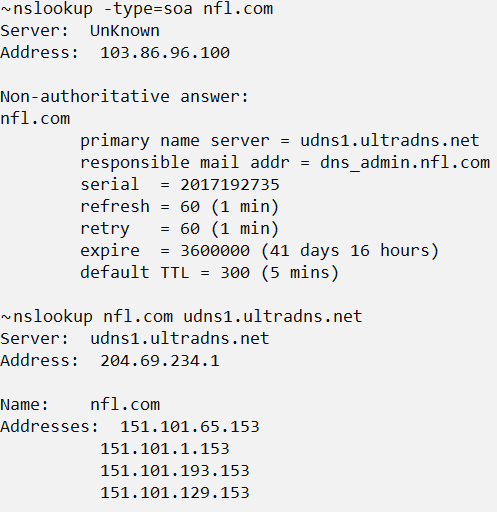
\includegraphics[width=300px]{assets/nslookup.png}
			\centering
			\caption{Obtaining the authoritative answer for the ip address of nfl.com}
		\end{figure}
			\clearpage
	\section{Problem - RSA}
		For the following RSA the values are selected
		\begin{itemize}
			\item $p=911$
			\item $q=883$
			\item $e=503$
		\end{itemize}
		\subsection{Describe these criteria for $e$ and $d$}
			To describe the criteria first the variable $n$ can be calculated.
			$$n=pq=911\cdot 883=804413$$
			Here $e<n$ and the greatest common divider between $e$ and $n$ must be 1.\\
			The criteria for $d$ is $ed\mod z = 1$ where $z=(p-1)(q-1)=910\cdot 882=802620$
		\subsection{Argue $e$ is a valid choice and calculate $d$ using the extended euclidean algorithm}
			It can be seen that $e<n\rightarrow 503 < 804413$ holds true\\
			To check if the greatest common divider between $e$ and $n$ is $1$, the euclidean algorithm can be used:
			\begin{align*}
				gcd(804413,503)\\
				804413 = 503\cdot 1599+116\\
				503=116\cdot 3+5\\
				116=5\cdot 23+1\\
				5=1\cdot 5+0\\
				gcd(804413,503)=1
			\end{align*}
			It can therefore be seen that $e$ is a valid choice for the algorithm since both criteria is fulfilled.\\
			To find a value $d$ the inverse euclidean algorithm can be performed
			\begin{align*}
				503d\mod 802620 = 1\\
				503d\equiv 1 \mod 802620\\
				d\equiv \frac{1}{503}\mod 802620\\
				d\equiv 503^{-1}\mod 802620\\
				\text{Using extended euclidean algorithm}\\
				802620=503\cdot 1595+335\\
				503=335\cdot 1 + 168\\
				335=168\cdot 1 + 167\\
				168=167\cdot 1 + 1\\[4mm]
				\text{Begin substituting}\\
				1=168-167\\
				1=168-(335-168)=168-335+168\\
				1=168\cdot 2 - 335\\
				1=(503-335)\cdot 2 - 335\\
				1=503\cdot 2 - 335 \cdot 3 \\
				1=503\cdot 2 - (802620-503\cdot 1595)\cdot 3\\
				1=503\cdot 2 - 802620\cdot 3 + 503\cdot 4785\\
				1=503\cdot 4787-802620\cdot 3\\
				1=503\cdot 4787\\[4mm]
				503^{-1}\equiv 4787 \mod 802620\\
				d=4787
			\end{align*} 
			It can be found that a valid value for $d$ is $4787$
		\subsection{Show how you can encrypt the number 3211. Show also how to decrypt your result}
			Encryption: $3211^e\mod n\rightarrow 3211^{503}\mod 804413=40516$\\
			Decryption: $40516^d\mod n\rightarrow 40516^{4787}\mod 804413=3211$
	\section{Problem - Modes of operation for Block Ciphers}
		Explain how each of these 5 modes of operation works.\\
		For the following explainations the following denotions are used:
		\begin{itemize}
			\item $C_i$ - Cipher for block $i$
			\item $p_i$ - Plaintext chunk $i$
			\item $c_i$ - Ciphertext chunk $i$
		\end{itemize}
		The cipher has the index, in case of use of a indexed key.
		\subsection{ECB}
			Electronic codebook (ECB) mode works by dividing the input into appropriate chunk size for the block cipher.\\
			Then each block is individually used as input for the block and the output will be the encrypted/decrypted text.\\
			$$ c_i =C_i(p_i)$$
			$$ p_i =C_i(c_i)$$
			The problem with this mode, is that in the case of duplicate chunks a pattern can be recognized.
		\subsection{CBC}
			Cipher Block Chaining (CBC) mode works by first a random $k$-bit string is generated called initialization vector (IV) and shared in plain text.\\
			Then the first block of input is XOR'ed with the IV. The following blocks is then XOR'ed with the last blocks output.\\
			$$c_0=C_0(p_0\oplus IV)$$
			$$ c_i = C_i(p_i\oplus c_{i-1})$$
			For the decryption the first block is decrypted an XOR'ed with the IV. Then the following blocks are decrypted and XOR'ed with the previous input block.
			$$p_0=C_0(c_0)\oplus IV$$
			$$p_i=C_i(c_i)\oplus c_{i-1})$$
		\subsection{CFB}
			Cipher Feedback (CFB) mode works by first a random $k$-bit string is generated called initialization vector (IV) and shared in plain text.\\
			The IV is then encrypted in the first block, and the output is XOR'ed with the first plain text chunk.\\
			The XOR result is then the first ciphertext chunk. For the following cipher block the previous XOR result is used for input to the next block and the output is XOR'ed with the next plain text chunk.
			$$c_0=C_0(IV)\oplus p_0$$
			$$ c_i = C_i( c_{i-1})\oplus p_i$$
			For the decryption first the IV is used as input for the block and the result is XOR'ed with the first cipher text chunk, which gives the first plain text chunk.\\
			For the following the ciphertext is used for input for the block and the result is XOR'ed with the next ciphertext chunk.
			$$p_0=C_0(IV)\oplus c_0$$
			$$ p_i = C_i( c_{i-1})\oplus c_i$$
		\subsection{OFB}
			Output Feedback (OFB) mode works by first a random $k$-bit string is generated called initialization vector (IV) and shared in plain text.\\
			This IV is then used as input for the first block cipher and the result is XOR'ed to create the cipher text.\\
			For the following ciphers the block cipher output from the previous block is used for input and the plaintext chunk is XOR'ed with the output to create the ciphertext.
			$$c_0=C_0(IV)\oplus p_0$$
			$$ c_i = C_i( c_{i-1}\oplus p_{i-1})\oplus p_i$$
			For this the decryption the same steps are repeated the only difference is the output of the block cipher is XOR'ed with the cipher text to create the plain text.
			$$p_0=C_0(IV)\oplus c_0$$
			$$p_i = C_i( p_{i-1}\oplus c_{i-1})\oplus c_i$$
			Note that for $c_i$ and $p_i$ the input to the cipher is the last ciphertext XOR'ed with the last plaintext which is equal to the last cipher output, but to simplify the equation and denotion the XOR cancellation is implicit.\\
		\subsection{CTR}
			Counter (CTR) mode works by first a random nonce is generated. Then a counter is initiated and synchronized between the encrypter and decrypter.\\
			The counter is then incremented for each block. The block then gets the sum of the nonce and counter as input. The output is the XOR'ed with the plaintext/ciphertext the encrypt/decrypt.\\
			$$c_i=C_i(\text{Nonce} + \text{counter})\oplus p_i$$
			$$p_i=C_i(\text{Nonce} + \text{counter})\oplus c_i$$
			The advantage of CTR is the ability to run parallel unlike CBC, CFB and OFB, where the input is dependent on the result of another cipher.
			
\end{document}
